\chapter{Results}\label{chap:results}
\section{Statistical brain shape analysis}

\begin{figure}[H]
	\centering
	\begin{center}
		\makebox[\textwidth]{\includesvg[width=0.95\paperwidth]{symmetryStats/STAGE00DATA/reduce10_gpaReps3/N_REP3/iters10000_nPicks5_perPickSize50_/results.svg}}
	\end{center}
	\caption[Statistical brain shape analysis results]{Asymmetry components significance analysis. Information about each landmark has been used to fill the \ac{3d} average shape of the left hemisphere, displayed medially and laterally. The \acp{mss} are produced by dividing \acp{rss} with the appropriate \acp{dof}. Both the first and the second column refer to information retrieved from the non-permuted data. The last column is derived by applying various thresholds (shown in the colorbar) on the p-value response presented on the third column.}
	\label{fig:stat_analysis}	
\end{figure}

Prior to the genetic studies, a statistical analysis purely on the phenotypic trait was done, to reveal existing symmetric patterns. The main results from the 2-way permutation \ac{anova} are summarized in \autoref{fig:stat_analysis} and are also being more formally medically followed by \citet{Vanbiervliet2022}. The individual effect (first row), which corresponds to the average shape variability across individuals, exhibits greater variation in the medial surface, particularly in the middle-anterior and middle-posterior parts of the cingulate gyrus and sulcus ($\subseteq$BA28, processing emotions and behavior regulation), the rostral part of the cuneus ($\subseteq$BA17, processing of visual information), the parahippocampal gyrus ($\subseteq$BA27, memory encoding and retrieval), and the fusiform gyrus ($\subseteq$BA37, recognition of faces). 

\Ac{da} (second row), the focus of this study, relevant to the general aptitude of individuals to exhibit certain asymmetric traits, is found to be highly significant in almost half of the studied surface. In line with the general identified asymmetry patterns presented in \autoref{subsec:general_sym_traits}, it is greatly localized around the peri-sylvian fissure and the temporal lobe (see peri-sylvian asymmetry). Also, it occurs in the medial surface, and the occipital lobe, implying relationship with the Yakovlevian torque, although lower significance of the effect is demonstrated on the prefrontal lobe.

\Ac{fa} effect (last row), which, as a reminder, is related to environmentally and developmentally induced variations, has been found generally significant across the cortical surface. This finding can be partly justified to the large combinatorial space from where permutations are collected (see \autoref{subsec:stat_methods}), as well as the overall exhibited plasticity of the human cortex (see \autoref{subsec:plasticity}), as raised by \citet{Vanbiervliet2022}. However, a comparison across regions is possible by inspecting  $F_{FA}$ instead, where, in the caudal part of the middle frontal gyrus ($\subseteq$ BA40, phonological processing and emotional responses), the superior part of the precentral gyrus ($\subseteq$ BA07, space localization), and the caudal part of the superior frontal sulcus and gyrus ($\subseteq$ BA08, planning complex movements) greater effect of \ac{fa} is exhibited.


\section{Covariates control}
The existing available metadata was used to exclude variability in the dataset that is not attributed to genetic factors. In \autoref{fig:covar}, the average covariates explained variance on each segment of \ac{dk} atlas is observed as retrieved from \ac{plsr}. The largest part of the frontal lobe, with greater impact on the inferior frontal, the inferior parietal gyrus and the parahippocampal gyrus appear to be more correlated with the collected metadata, shown in \autoref{tab:covariates}. The results point to less observed explained variation around the area of the sylvian fissure and the temporal lobe, and also raise a degree of uncertainty on the significant response observed during the statistical shape asymmetry analysis, regarding the medial surface and the inferior part of the frontal lobe.
\begin{figure}[H]
\includesvg[width=0.9\textwidth]{asymmetry/hierarchicalClusteringDemo/STAGE00DATA/asymmetry_reduction1/explainedDKCovariates.svg}
\caption[Explained variance from covariates]{Explained variance from the covariates on each \ac{dk} atlas segment, as retrieved from \ac{plsr}, mapped on the average left hemisphere medial and lateral side.}
\label{fig:covar}
\end{figure}
\section{Partitioning and \acs{pca}}

To perform a coarse-to-fine analysis,  \ac{hsc} was applied on the preprocessed phenotype. In \autoref{fig:partitioning}, the partitioning produced from the application of \ac{hsc} is displayed. On the first level, although the cross-section accurately follows the sylvian fissure on the lateral part and partitions the frontal lobe from the rest of the hemisphere, on the medial surface it appears to split the precuneus in half ($\subseteq$ BA07). On the second level, the occipital lobe is separated from the temporal lobe, while the central gyrus appears to be dissected from the frontal lobe, while inspected the lateral surface. On the medial surface, the paracentral gyrus ($\subseteq$ BA04)is approximately separated from the superior-frontal, whereas another cross section appears to share its boundaries with the temporal pole ($\subseteq$ BA38). In general, the unsupervised clustering follows the functional partitioning, validating the close relationship  between function and morphology of each cortical region. The calculated \ac{nmi} score for the partitioning, compared to the \ac{dk} atlas is displayed in \autoref{tab:nmi} for each level. Although the finer the partitioning, the further away from the theoretical maximum value, quantitatively the two clusterings highly agree.

\begin{figure}[H]
	\begin{adjustwidth}{-4cm}{-4cm}
	\centering
	\subfloat[]{
		\includesvg[width=0.6\linewidth]{asymmetry/hierarchicalClusteringDemo/STAGE00DATA/asymmetry_reduction1/levels4/segmentation.svg}
	}\quad
	\subfloat[]{
		\includesvg[width=0.4\linewidth]{asymmetry/hierarchicalClusteringDemo/STAGE00DATA/asymmetry_reduction1/levels4/segmentation_circular.svg}
	}

\end{adjustwidth}
\caption[4-level brain shape partitioning based on asymmetry]{4-level brain shape partitioning based on cortical asymmetry, using \ac{hsc}. Shown in 2 different versions, on a level representation (top), and as a polar dendrogram plot, annotated with white color against black background (bottom). Those representations are used across the coarse-to-fine analysis in this study.}
\label{fig:partitioning}
\end{figure}

\begin{table}[H]
	\centering
	\begin{tabular}{l|ccc}
		& NMI & $\NMI_{max}$ & ratio\\
		\hline
		 Lvl 1 & 0.37 & 0.48 & 0.78\\
		 Lvl 2 & 0.49 & 0.66 & 0.74\\
		 Lvl 3 & 0.55 & 0.79 & 0.71\\
		 Lvl 4 & 0.62 & 0.90 & 0.69\\
	\end{tabular}
\caption [\Ac{nmi} scores across \ac{hsc} partitioning levels]{\Ac{nmi} scores across \ac{hsc} partitioning levels, comparing \ac{dk} atlas with computed partitioning levels. $\NMI_{max}$ is an approximate maximal value, given the different number of partitions in each clustering, and ratio is the scaled \ac{nmi} using that value.}
\label{tab:nmi}
\end{table}
The required number of \ac{pca} features per partition given the constraints, as computed by assessing the discovery dataset, is displayed in \autoref{fig:pcs_num}. A significant dimensionality reduction was achieved, given that the original total number of landmark coordinates per individual was 89367.
\begin{figure}[H]
\includesvg[width=0.9\textwidth]{asymmetry/hierarchicalClusteringDemo/STAGE00DATA/asymmetry_reduction1/levels4/explainedVarianceSIngleThreshold.svg}
\caption[Number of PCs per HSC cortical surface partition]{Number of \acp{pc} for each \ac{hsc} cortical surface partition, required to explain 80\% of its variance, relatively to the discovery dataset. For the first partition, the upper limit of 500 components was reached and only 74\% of its variance is explained.}
\label{fig:pcs_num}
\end{figure}
\section{\acs{gwas}}
By combining the aforementioned processed phenotypic and genetic features under the framework of \ac{cca}, insights were provided into the genetics of asymmetry. The resulting \ac{mvgwas} Manhattan plot on the entire hemisphere exhibits distinct peaks, that slightly differ between discovery and replication dataset (\autoref{fig:entire_gwas}). In \autoref{tab:leadsnps}, the identified \acp{snp} are shown for the discovery and replication datasets \acp{gwas}, as well as the meta-analysis \ac{gwas} union and the ones reported in literature \cite{Sha2021}. Additionally, the number of significant variants after Bonferroni correction is reported in \autoref{fig:part_bonferroni}, with the overlaid Manhattan plots shown  in \autoref{fig:part_manhattan}. 

A different chromosome-based response is observed when inspecting the second level of partitioning, namely partitions 4-7, so a further analysis has been deemed necessary on each of those partitions separately. Furthermore, partition 6, which corresponds to the frontal lobe cortical asymmetry, appears to be quite less genetically determined and agrees with the findings from the statistical analysis, where \ac{da} did not appear to be, in general, significant in that region, whereas \ac{fa} did (\autoref{fig:stat_analysis}). An additional observation is that partitions do not necessarily share the genetic signature of their parents, for example partition 8 exhibits a significant peak at chromosome 21, while that chromosome has not been identified elsewhere to exhibit significant genetic effect on cortical asymmetry.  Chromosome 15 exhibits the highest peak, namely the \ac{snp} rs2033939 (P=2e-50). 

To confirm that mean substitution of missing genotypes (i.e, variants that, even after imputation, had not been assigned a value) did not considerably affect the results, Spearman correlation was measured between the \ac{gwas} scores produced from the discovery dataset, with and without mean substitution. The produced values clearly suggested that mean substitution had little to no effect on the overall monotonicity (table \autoref{tab: spearman_no_vs_mean}).

\begin{adjustwidth}{-3 cm}{-2.5 cm}\centering\begin{threeparttable}[!htb]	
		\scriptsize
		\begin{tabular}{ccc||ccc||ccc||ccc}\toprule
			\multicolumn{3}{c}{\textbf{DISCOVERY}} &\multicolumn{3}{c}{\textbf{REPLICATION}} &\multicolumn{3}{c}{\textbf{UNION}} &\multicolumn{3}{c}{\textbf{SHA ET AL.}} \\\midrule
			\textbf{CHR} &\textbf{SNP} &\textbf{P} &\textbf{CHR} &\textbf{SNP} &\textbf{P} &\textbf{CHR} &\textbf{SNP} &\textbf{P} &\textbf{CHR} &\textbf{SNP} &\textbf{P} \\
			15 &rs1080066 &4.10e-28 &15 &rs4924345 &1.41e-27 &15 &rs2033939 &2.09e-50 &10 &\textbf{rs41298373} &5.00e-38 \\
			17 &rs10775404 &5.12e-27 &17 &rs9910683 &2.42e-20 &17 &17:44243312\_C\_G &3.91e-44 &17 &rs35853889 &1.00e-20 \\
			14 &rs160459 &2.57e-17 &9 &rs7023465 &3.74e-18 &14 &\textbf{rs160459} &3.58e-28 &17 &rs80103986c &5.00e-16 \\
			1 &rs6658111 &3.05e-15 &14 &rs74826997 &3.02e-14 &9 &rs7023465 &1.40e-25 &9 &rs911934 &2.00e-15 \\
			16 &rs111398992 &1.17e-12 &14 &rs160459 &6.57e-13 &1 &\textbf{rs6658111} &4.31e-25 &17 &rs55938136 &5.00e-15 \\
			2 &rs7575465 &1.57e-12 &1 &rs6658111 &8.08e-12 &14 &rs74826997 &3.36e-22 &16 &\textbf{rs111398992} &6.00e-15 \\
			16 &rs9939914 &7.01e-12 &10 &rs41298373 &2.10e-11 &16 &\textbf{rs72813426} &3.78e-21 &17 &rs568039055 &8.00e-15 \\
			10 &rs41298373 &3.66e-11 &16 &rs35769864 &1.40e-10 &10 &\textbf{rs41298373} &9.26e-21 &16 &\textbf{rs72813426} &2.00e-14 \\
			17 &rs62063672 &1.40e-10 &12 &rs10783306 &7.41e-10 &16 &\textbf{rs111398992} &1.66e-20 &14 &\textbf{rs160459} &5.00e-12 \\
			3 &rs35124509 &2.71e-10 &2 &rs7575465 &7.75e-10 &2 &rs7575465 &1.80e-20 &12 &rs10783306 &1.00e-11 \\
			14 &rs76341705 &3.81e-10 &16 &rs111398992 &9.24e-10 &3 &rs35124509 &1.26e-15 &2 &rs12617392 &4.00e-11 \\
			9 &rs911934 &4.71e-10 & & & &16 &rs11640500 &2.84e-15 &1 &\textbf{rs6658111} &1.00e-10 \\
			3 &rs2399037 &4.21e-9 & & & &12 &rs1057548 &1.71e-13 &2 &rs62130503 &1.00e-10 \\
			7 &rs117766132 &6.39e-9 & & & &16 &rs12711472 &4.61e-12 &2 &rs368536282 &1.00e-10 \\
			\cellcolor[HTML]{C8C8C8}2 &\cellcolor[HTML]{C8C8C8}rs2691112 &\cellcolor[HTML]{C8C8C8}1.29e-8 & & & &2 &rs7601767 &8.67e-11 &6 &rs7781 &2.00e-10 \\
			\cellcolor[HTML]{C8C8C8}2 &\cellcolor[HTML]{C8C8C8}rs7601767 &\cellcolor[HTML]{C8C8C8}1.88e-8 & & & &7 &rs151218739 &1.76e-10 &14 &rs201816193 &4.00e-10 \\
			\cellcolor[HTML]{C8C8C8}8 &\cellcolor[HTML]{C8C8C8}rs7000137 &\cellcolor[HTML]{C8C8C8}2.60e-8 & & & &8 &rs10106820 &1.80e-10 &19 &rs11672092 &6.00e-10 \\
			& & & & & &2 &rs13021393 &6.80e-10 &21 &\textbf{rs7283026} &8.00e-10 \\
			& & & & & &21 &\textbf{rs7283026} &3.01e-9 &3 &rs2279829 &1.00e-9 \\
			& & & & & &8 &rs442103 &3.43e-9 &5 &rs869219775 &3.00e-9 \\
			& & & & & &15 &rs8026370 &4.49e-9 &20 &rs6135555 &7.00e-9 \\
			& & & & & &21 &rs4819075 &5.01e-9 &\cellcolor[HTML]{C8C8C8}X &\cellcolor[HTML]{C8C8C8}rs12400461 &\cellcolor[HTML]{C8C8C8}1.00e-8 \\
			& & & & & &\cellcolor[HTML]{C8C8C8}2 &\cellcolor[HTML]{C8C8C8}rs2287283 &\cellcolor[HTML]{C8C8C8}1.38e-8 &\cellcolor[HTML]{C8C8C8}6 &\cellcolor[HTML]{C8C8C8}rs9385385 &\cellcolor[HTML]{C8C8C8}1.00e-8 \\
			& & & & & &\cellcolor[HTML]{C8C8C8}2 &\cellcolor[HTML]{C8C8C8}rs7609463 &\cellcolor[HTML]{C8C8C8}1.38e-8 &\cellcolor[HTML]{C8C8C8}17 &\cellcolor[HTML]{C8C8C8}rs35908989 &\cellcolor[HTML]{C8C8C8}1.00e-8 \\
			& & & & & &\cellcolor[HTML]{C8C8C8}17 &\cellcolor[HTML]{C8C8C8}rs930119 &\cellcolor[HTML]{C8C8C8}3.02e-8 &\cellcolor[HTML]{C8C8C8}4 &\cellcolor[HTML]{C8C8C8}rs9307052 &\cellcolor[HTML]{C8C8C8}2.00e-8 \\
			& & & & & &\cellcolor[HTML]{C8C8C8}11 &\cellcolor[HTML]{C8C8C8}rs2251662 &\cellcolor[HTML]{C8C8C8}3.41e-8 &\cellcolor[HTML]{C8C8C8}22 &\cellcolor[HTML]{C8C8C8}rs9615351 &\cellcolor[HTML]{C8C8C8}3.00e-8 \\
			& & & & & & & & &\cellcolor[HTML]{C8C8C8}7 &\cellcolor[HTML]{C8C8C8}rs6947352 &\cellcolor[HTML]{C8C8C8}4.00e-8 \\
			\bottomrule
		\end{tabular}
		\caption[Identified lead \acp{snp} for the entire hemisphere]{Identified lead \acp{snp} for the entire hemisphere across the different datasets, along with a comparison with \citet{Sha2021}. In gray, \acp{snp} with significance less than 1e-8 but greater than 5e-8 are reported. In bold are displayed the variants identified both in the present study and in the work of \citet{Sha2021}.}
		\label{tab:leadsnps}
\end{threeparttable}\end{adjustwidth}

\begin{figure}[H]
	\centering
	\subfloat{
		\includesvg[width=1\textwidth]{asymmetry/genomeDemo/STAGE00DATA/mean_imputed/not_subsampled/gwas_discovery.svg}
	}
	\par\medskip
	\centering
	\subfloat{
		\includesvg[width=1\textwidth]{asymmetry/genomeDemo/BATCH2_2021_DATA/mean_imputed/not_subsampled/gwas_replication.svg}	
	}
	\par\medskip
	\centering
	\subfloat{
		\includesvg[width=1\textwidth]{asymmetry/meta_analysis/joinedDatasets/mean_imputed/not_subsampled/gwas_joined.svg}	
	}
	\caption[mvGWAS of the entire hemisphere shape asymmetry]{\Ac{mvgwas} of the entire hemisphere shape asymmetry computed on the discovery (top) and the replication (middle) dataset, along with the meta-analysis union based on Stouffer's method (bottom). The genome-wide threshold of 5e-8 is also being displayed as a horizontal line.}
	\label{fig:entire_gwas}
\end{figure}


\begin{figure}[H]
	\begin{adjustwidth}{-4cm}{-3cm}
	\centering
	\subfloat{
		\includesvg[width=0.95\linewidth]{asymmetry/visualizeCCAOnPheno/joinedDatasets/mean_imputed/not_subsampled/WithBC/CcaCircularJoined.svg}
	}
	\subfloat{
		\includesvg[width=0.05\linewidth]{asymmetry/visualizeCCAOnPheno/joinedDatasets/mean_imputed/not_subsampled/WithBC/legend.svg}
	}
	\end{adjustwidth}	
	\caption[Number of significant SNPs after Bonferroni correction along partitions]{Number of significant \acp{snp} per chromosome after Bonferroni correction across partitions. The variants number per chromosome is shown inside boxes of a different color, as displayed in the legend on the right.}
	\label{fig:part_bonferroni}
\end{figure}

\section{\acs{ldsr}}
\label{sec:ldsr_results}
Another important question to be answered was how much of the variability of cortical symmetry is attributed to genetic factors. The observed heritability is generally below 0.3 across the different partitioning levels (figure \autoref{fig:herit_part}), as expected from the effect of plasticity on human cortex. The heritability estimates minima and maxima grossly agree with the results of \citet{Sha2021}. Comparably more heritable than in other regions appears to be the asymmetry on the temporal lobe, on the auditory cortex and the basal surface of the temporal lobe.  The confounding bias is found to be considerably low, with the \ac{ldsr} intercept being close to 1 \cite{Bulik-Sullivan2015} (figure \autoref{fig:confbias}), so little to no evidence is presented regarding subpopulation stratification. 


\section{Cross-traits correlation}
\label{sec:ct-res}
To examine whether cortical asymmetry is genetically related with other indications, and potentially reason about the universal patterns among individuals, statistical tests for cross-trait monotonicity followed. After performing Spearman correlation with the univariate traits mentioned in \autoref{subsec:other_sources}, no monotonicity between cortical asymmetry p-values and the \ac{gwas} scores of the following traits was identified:
\begin{itemize}
	\item{\Acf{adhd}}
	\item{\Acf{asd}}
	\item{\Acf{ad}}
	\item{\Acf{bd}}
	\item{Major Depressive Disorder}
	\item{Schizophrenia}
\end{itemize}



\begin{figure}[H]
	\centering
	\subfloat[Scaled heritability]{
	\includesvg[width=5.5cm]{asymmetry/visualizeHeritabilityOnPheno/joinedDatasets/mean_imputed/not_subsampled/Total Observed scale h2.svg}
	\label{fig:herit_part}
	}
	\quad
	\subfloat[\Ac{ld} score intercept]{
		\includesvg[width=5.5cm]{asymmetry/visualizeHeritabilityOnPheno/joinedDatasets/mean_imputed/not_subsampled/Intercept.svg}
		\label{fig:confbias}
	}
	\caption[LDSR results across partitioning levels]{\Ac{ldsr} results on the entire hemisphere and each partitioning level.}
	\label{fig:ldsr}
\end{figure}


By inspecting the results from Spearman cross-trait correlation (\autoref{fig:spearmanOtherTraits} and \ref{fig:cross_trait_polar}), language functional connectivity exhibits the strongest relationship, for the entire hemisphere and partition 17.  Educational attainment also appears to be strongly correlated with cortical asymmetry, with the strongest sign occurring on the 2\textsuperscript{nd} partition, which includes most sensory areas. \Ac{ocd} exhibits strong correlation with cortical asymmetry with partitions 14 and 26. 
Partition 11 from the 3rd level and its child partition 22 from the 4th level point to correlation with handedness. Furthermore, intelligence exhibits significant genetic correlation with partitions 9 and 11, both exhibiting \ac{gwas} peaks on chromosomes 9 and 15 (\autoref{fig:part_bonferroni}).

Investigating the relations of cortical asymmetry with another trait related to cortical structure, specifically the average mid-cortical surface per individual, coined as brain shape, and the corresponding 8-level \ac{hsc} partitioning and \ac{gwas} performed by \citet{Naqvi2021} in a similar fashion to the present study, it is apparent from \autoref{fig:spearmanShape} that there is a quite strongly supported genetic relationship. Such correlation stands not only for the entire hemisphere (partition 1 and shap1 respectively), but also for other pairs, with observed P-values getting as low as 10e-59, and Spearman correlation values as high as 0.34.





\begin{figure}[H]

	\subfloat[Spearman Correlation]{
		\includesvg[width=.5\textwidth]{asymmetry/spearman_correlation/joinedDatasets/mean_imputed/not_subsampled/other_traits/otherTraitsHeatmap.svg}}
	\subfloat[Bootstrapping P-value]{
		\includesvg[width=.5\textwidth]{asymmetry/spearman_correlation/joinedDatasets/mean_imputed/not_subsampled/other_traits/otherTraitsHeatmapPvalues.svg}}
	\caption{Cross-trait correlation stats across partitions in a tabular format.}
	\label{fig:spearmanOtherTraits}
	
\end{figure}

\begin{figure}[H]
\begin{adjustwidth}{-3cm}{-3cm}
	\subfloat[Spearman Correlation]{
		\includesvg[width=\linewidth]{asymmetry/spearman_correlation/joinedDatasets/mean_imputed/not_subsampled/brain_shape/brainShapeHeatmap.svg}}
	\par\medskip
	\subfloat[Bootstrapping P-value]{
		\includesvg[width=\linewidth]{asymmetry/spearman_correlation/joinedDatasets/mean_imputed/not_subsampled/brain_shape/brainShapeHeatmapPvalues.svg}}
	\caption[Brain shape genetically related to cortical asymmetry]{Brain shape partitions (x-axis) \ac{gwas} scores, as derived by \citet{Naqvi2021}, compared against cortical asymmetry partitions (y-axis) \ac{gwas} scores of the present study.}
	\label{fig:spearmanShape}
\end{adjustwidth}
\end{figure}


\begin{figure}[H]
	\begin{adjustwidth}{-4cm}{-3cm}
		\centering
		\subfloat{
			\includesvg[width=0.9\linewidth]{asymmetry/spearman_correlation/joinedDatasets/mean_imputed/not_subsampled/other_traits/otherTraits/CcaCircularOtherTraits.svg}
		}
		\subfloat{
			\includesvg[width=0.1\linewidth]{asymmetry/spearman_correlation/joinedDatasets/mean_imputed/not_subsampled/other_traits/otherTraits/otherTraitsLegend.svg}
		}
	\end{adjustwidth}	
	\caption[Cross-trait correlation with cortical asymmetry in a polar diagram]{Cross-trait correlation with asymmetry in a polar diagram. Only correlations with p-values less than 0.05 are shown.}
	\label{fig:cross_trait_polar}
\end{figure}


\section{\acs{ldsc-seg}}
After having determined the genetic factors that drive cortical asymmetry, it is of interest to examine the amount of epigenetic regulation affecting them, by investigating profiles of different types of tissues. In \autoref{fig:ldsc-seg-chromatin} chromatin accessibility enriched regions for specific adult or developing tissues were found to be related with cortical asymmetry heritability. Out of the 489 tested tissues, mainly those related with the brain, and in particular with the fetal brain, exhibited more significant relationship with the studied population. The strongest significance was displayed by the fetal brain female tissue, versus the male analog, suggesting that female fetuses may exhibit increased asymmetric heritability. However, these results need to be taken with a grain of salt, as the underlying population used to collect the samples was comprised only by a few individuals, at different time periods, so it is quite possible that uncontrollable factors and sample bias obscure the results. Another observation is that partitions that `reacted` to this analysis are mainly localized on regions that had already been found to have increased heritability in \autoref{sec:ldsr_results} and figure \autoref{fig:herit_part}.


\begin{figure}[H]
	\begin{adjustwidth}{-3cm}{-3cm}
	\centering
	\includesvg[width=\linewidth]{asymmetry/ldsc/joinedDatasets/mean_imputed/not_subsampled/h2-cts/Multi_tissue_chromatin/ldsc_seg_pHeatmap_chromatin.svg}
	\caption[LDSC-SEG assessment on variable chromatin accessibility]{Significance of heritability affected by different tissues enriched chromatin accessibility profiles, across partitions. Unavailable(white) values and missing partitions mean that the \ac{ldsc-seg} algorithm failed to identify strong relationships in these cases. H3K27ac, H3K4me3 and HeK4me1 are each different epigenetic modifications on histones, the molecules that compose the \ac{dna} packaging, and are used as markers of gene regulation.}
	\label{fig:ldsc-seg-chromatin}
	\end{adjustwidth}
\end{figure}
\section{Developmental analysis}
For the following analyses, only the \ac{gwas} scores produced by assessing the entire hemisphere and the 2\textsuperscript{nd} level partitions are assessed. In \autoref{fig:age_dev}, genetic loci that have been found strongly in connection with the existence of cortical asymmetry appear to be developmentally regulated, with their activity primarily detected in the early weeks of gestation, while the stringent regulatory mechanism, which is activated after the 2\textsuperscript{nd} month of gestation, appears to `relax` during adolescence. The variability of the regulatory pattern on different partitions does infer that not all structural characteristics develop at the same time across the human cortex.

\begin{figure}[H]
	\begin{adjustwidth}{-3cm}{-3cm}
	\centering
	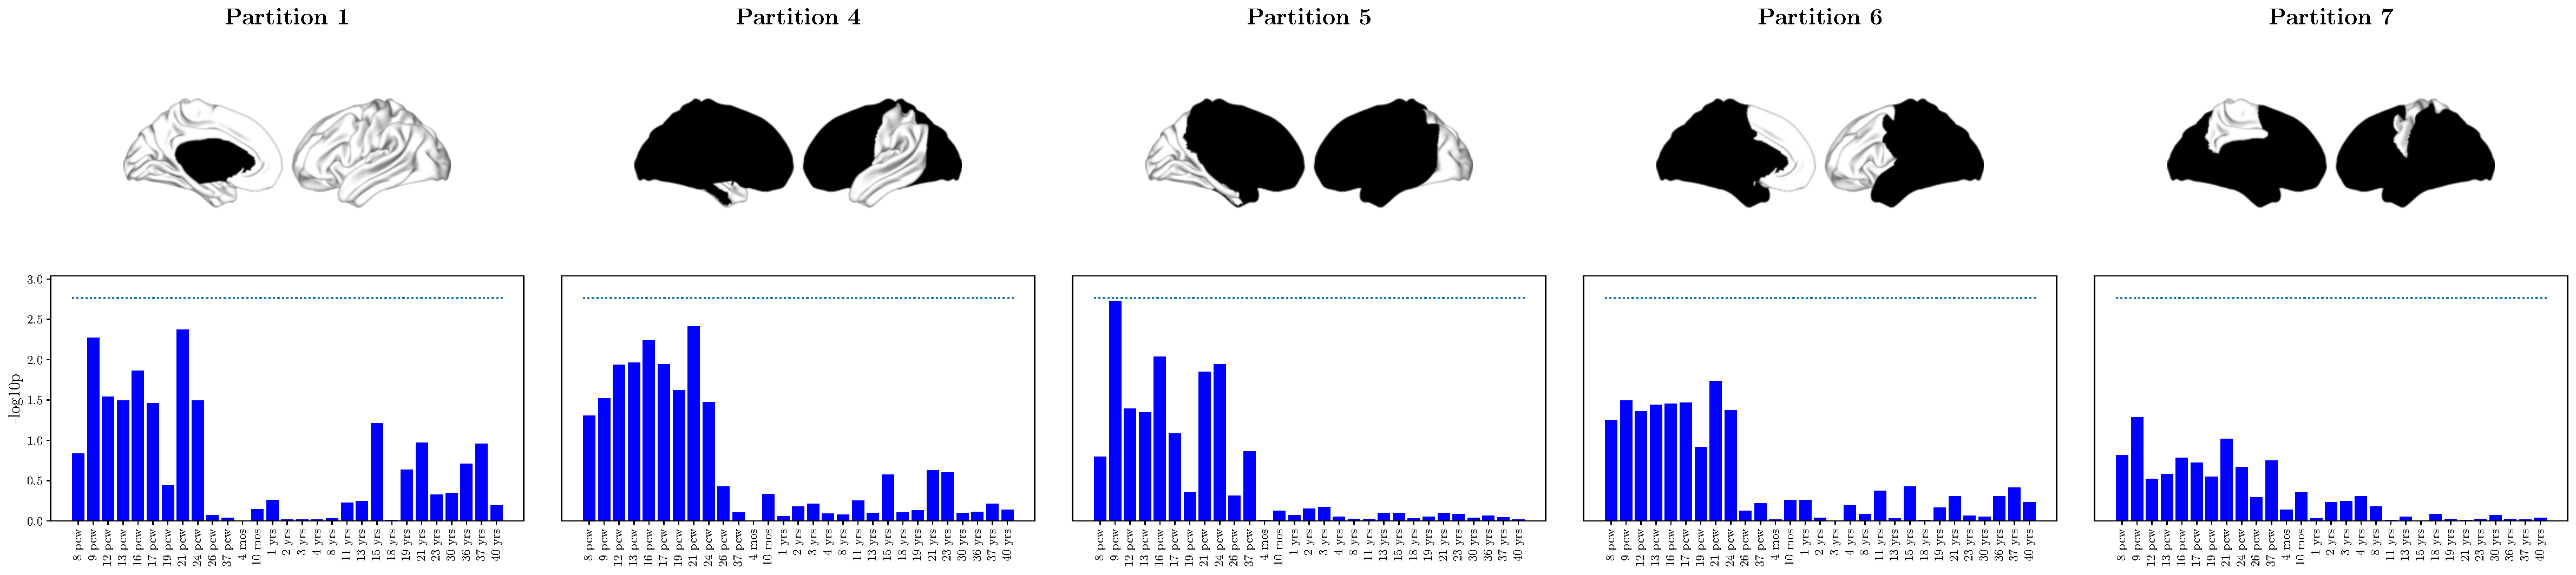
\includegraphics[width=0.8\linewidth]{asymmetry/FUMA/joinedDatasets/mean_imputed/not_subsampled/partitionsSummary/age}
	\caption[Brain tissue specific age enriched genes analysis]{MAGMA analysis on age specific brain tissue enriched genes, on the \acp{gwas} of the entire hemisphere and the 2\textsuperscript{nd} level partitions.}
	\label{fig:age_dev}
	\end{adjustwidth}
\end{figure}


\begin{adjustwidth}{-3 cm}{-3 cm}\centering\begin{threeparttable}[H]
	\tiny
	\begin{tabular}{ccc||cc||ccc||c||cc}\toprule
		\multicolumn{3}{c}{\textbf{Partition 1}} &\multicolumn{2}{c}{\textbf{Partition 4}} &\multicolumn{3}{c}{\textbf{Partition 5}} &\textbf{Partition 6} &\textbf{Partition 7} \\
		\multicolumn{3}{c}{\textbf{84 genes}} &\multicolumn{2}{c}{\textbf{43 genes}} &\multicolumn{3}{c}{\textbf{68 genes}} &\textbf{32 genes} &\textbf{34 genes}
		\\\midrule
		AGBL5 &FOXD2 &\textbf{SHFM1} &\textbf{ALCAM} &RP11-368I7.4 &\textbf{ACTR10} &GAS8 &TIMM9 &ARL17A &ARL17A \\
		ARL17A &\textbf{FOXL1} &\textbf{SLA} &ARL17A &SFMBT2 &AGBL5 &ITIH5 &TMEM214 &ARL17B &ARL17B \\
		ARL17B &\textbf{FOXN2} &\textbf{SLC25A13} &ARL17B &SPATA33 &\textbf{ARHGAP27} &KANSL1 &\textbf{TOMM20L} &C17orf58 &C16orf3 \\
		C16orf3 &GALNT12 &SPATA33 &C16orf3 &SPIRE2 &ARL17A &\textbf{KCNA5} &TRABD2B &CRHR1 &C17orf58 \\
		\textbf{C16orf95} &GAS8 &SPATS2 &C17orf58 &SPPL2C &ARL17B &KHK &TUBB3 &DHH &CENPBD1 \\
		CDK10 &ITIH5 &SPIRE2 &CENPBD1 &STH &C16orf3 &L3HYPDH &VPS9D1 &DNAJC22 &CRHR1 \\
		CENPBD1 &KANSL1 &SPRED2 &COL15A1 &TCF25 &C17orf58 &\textbf{LHCGR} &WNT3 &FMNL3 &DAAM1 \\
		CGREF1 &KHK &\textbf{STRN} &COL18A1 &THBS1 &CDK10 &\textbf{LHPP} &ZNF276 &\textbf{GTF2A2} &DBNDD1 \\
		CHMP1A &KMT2D &TCF25 &CRHR1 &TIMM9 &CENPBD1 &LRRC37A & &KANSL1 &DEF8 \\
		CMPK1 &LMBR1L &\textbf{TENM4} &DAAM1 &TUBB3 &CGREF1 &LRRC37A2 & &KMT2D &FANCA \\
		COL15A1 &LRRC37A &THBS1 &DACT1 &VPS9D1 &CHMP1A &\textbf{LRRC37A3} &\textbf{} &LMBR1L &GAS8 \\
		COL18A1 &LRRC37A2 &TIMM9 &DBNDD1 &WNT3 &CMPK1 &MAPRE3 & &LRRC37A &KANSL1 \\
		CPNE7 &LYPD6 &TMBIM6 &DEF8 &ZNF276 &COL15A1 &MAPT & &LRRC37A2 &L3HYPDH \\
		CRHR1 &LYPD6B &TMEM214 &EPHA3 & &CPNE7 &MC1R & &\textbf{MAP2} &LRRC37A \\
		DAAM1 &MAPRE3 &TRABD2B &FANCA & &CRHR1 &\textbf{METTL10} &\textbf{} &MAPT &LRRC37A2 \\
		DACT1 &MAPT &TROAP &GALNT12 & &DAAM1 &\textbf{NR2F1} &\textbf{} &MC1R &MAPT \\
		DBNDD1 &MC1R &TUBA1A &GAS8 & &DACT1 &NSF & &MEIS1 &MC1R \\
		DEF8 &MEIS1 &TUBA1B &ITIH5 & &DBNDD1 &\textbf{NTF3} &\textbf{} &NSF &NSF \\
		DHH &NSF &TUBA1C &KANSL1 & &DEF8 &OST4 & &PRKAG1 &\textbf{rs4924345} \\
		\textbf{DLX6} &OST4 &TUBB3 &\textbf{KCNK16} &\textbf{} &DPYSL5 &PLEKHM1 & &RHEBL1 &\textbf{rs7023465} \\
		DNAJC22 &PLEKHM1 &\textbf{VIT} &\textbf{KIF6} &\textbf{} &EMILIN1 &PREB & &SPATS2 &\textbf{rs72813426} \\
		\textbf{DPYSL2} &\textbf{PNMA2} &\textbf{WISP1} &LRRC37A & &EPHA3 &\textbf{RP11-12J10.3} &\textbf{} &SPPL2C &\textbf{rs75267789} \\
		DPYSL5 &POFUT2 &WNT3 &LRRC37A2 & &\textbf{FAM175B} &RP11-368I7.4 & &SPRED2 &\textbf{rs76341705} \\
		EMILIN1 &PREB &ZNF276 &LYPD6 & &\textbf{FAM53B} &RTN1 & &STH &RTN1 \\
		EPHA3 &PRKAG1 & &LYPD6B & &FANCA &SFMBT2 & &TCF25 &SPATA33 \\
		FANCA &\textbf{QPCT} &\textbf{} &MAPT & &\textbf{FMNL1} &SPATA33 & &TMBIM6 &SPIRE2 \\
		\textbf{FBXO11} &RASGRP1 & &MC1R & &\textbf{FNDC4} &SPIRE2 & &TROAP &SPPL2C \\
		\textbf{FBXO31} &RHEBL1 & &NSF & &FOXD2 &SPPL2C & &TUBA1A &STH \\
		FMNL3 &RP11-368I7.4 & &POFUT2 & &\textbf{FSHR} &STH & &TUBA1B &TCF25 \\
		\textbf{FOXC2} &RTN1 & &RASGRP1 & &GALNT12 &TCF25 & &TUBA1C &THBS1 \\
		& & & & & & & &\textbf{UNC80} &TUBB3 \\
		& & & & & & & &WNT3 &VPS9D1 \\
		& & & & & & &\textbf{} & &WNT3 \\
		& & & & & & & & &ZNF276 \\
		\bottomrule
	\end{tabular}
	\caption[Identified gene sets]{Identified gene sets using FUMA and GREAT for the entire hemisphere and the 2\textsuperscript{nd} level partitioning \acp{gwas}. In bold, the genes that do not occur in other gene sets are displayed. Lead \acp{snp} that have not been mapped to a gene are also displayed with their rs-id.}
	\label{tab:genesets}
\end{threeparttable}\end{adjustwidth}


\section{Functional association}
\label{sec:res_functional}
The extrapolation of the identified lead \acp{snp} to the gene abstraction level, using FUMA and GREAT produced the genes sets presented in \autoref{tab:genesets}. It is evident that there are differences, and even certain genes appear to be related with cortical asymmetry only in certain partitions. By examining FUMA functional association with \ac{go} terms, a tight connection of the identified gene set is demonstrated with the cytoskeleton and particularly with the microtubules function and biological processes (\autoref{fig:go} and \ref{fig:go_genes}), in line with literature \cite{Sha2021}. Furthermore, testing the identified gene set versus gene differential expression of diverse tissues, cerebral and cerebellum tissues displayed the greatest enrichment (\autoref{fig:de_genes}), whereas thyroid and female gender related tissues, namely uterus and ovary ones, exhibit mostly downregulated genes enrichment. By investigating the gene set enrichment on traits reported in \ac{gwas} catalog (\autoref{fig:gw_catalog} and \ref{fig:gw_catalog_genes}), behavior-related traits, such as alcohol use disorder, handedness, and phenotypic traits closely related to the exoderm, such as sun tan response, male baldness and the red hair trait, appear highly correlated with the identified asymmetry gene sets. Canonical pathways enrichment analysis (\autoref{fig:can_pathways} and \ref{fig:can_pathways_genes}) reveals connections with NMDA receptors pathways, particularly on the frontal lobe,  known to control synaptic plasticity and memory function in mammals \cite{Li2009}.

\section{Proteins set network analysis}

Last but not least, through the analysis of the computed STRING proteins network on the \ac{gwas} of the entire hemisphere, densely connected clusters were identified and their functional identity was researched through gene enrichment analysis (\autoref{fig:string_net}). The results showcase four main pathways, governing cytoskeleton formation at diverse abstraction levels, with the first cluster related to the \ac{lr} axis formation \cite{Hu2017}, the second cluster to the \ac{dv} axis formation \cite{Hikasa2013}, the third participating in the intracellular cytoskeleton structure and the fourth in the extracellular matrix formation. However, it is worth noting that the degree of enrichment is succinct, because if any correction is applied by PANTHER software most clusters are not mapped to a specific pathway. Enriched publications identified were mainly related to chromosome 17 and Koolen de Vries syndrome, a genetic disease that is being identified in \ac{mri} scan as highly asymmetric ventricles, that in many cases gives rise to increased cortical asymmetry \cite{Myers2017}.

\begin{figure}[H]
\begin{adjustwidth}{-3cm}{-3cm}
	\begin{minipage}{0.5\linewidth}
		\centering
		\includesvg[inkscapelatex=false, width=\textwidth]{asymmetry/STRING/joinedDatasets/par01/clusterMCL2.svg}
	\end{minipage} \quad
	\begin{minipage}{0.5\linewidth}
		\subfloat[Cluster 1, 13 genes participating in Hedhegog gene signalling (Reactome GO enrichment through Panther without correction, with Fisher's exact test, P-value=1e-2).]{
			\includesvg[pretex=\tiny, width=0.4\textwidth]{asymmetry/STRING/joinedDatasets/par01/clusterMCL2_1/clusterMCL2_1.svg}
		}
	\quad
	\subfloat[Cluster 2, 8 genes participating in WNT ligand biogenesis, to regulate morphogenesis, namely the positioning of different cell types in a tissue during development (P-value={9e-3}).]{
		\includesvg[pretex=\tiny, width=0.4\textwidth]{asymmetry/STRING/joinedDatasets/par01/clusterMCL2_2/clusterMCL2_2.svg}
	}
	\par\medskip
	\subfloat[Cluster 3, 8 genes with a role in gap junction assembly(P-value=1e-10), activation of AMPK downstream of NMDARs (P-value=4e-13) and tubulin folding(P-value=2e-10).]{
	\includesvg[pretex=\tiny, width=0.4\textwidth]{asymmetry/STRING/joinedDatasets/par01/clusterMCL2_3/clusterMCL2_3.svg}
	}\qquad	
	\centering	
	\subfloat[Cluster 4, 5 genes participating in extracellular matrix organization, specifically in collagen formation (P-value=2e-4), but also in its degradation (P-value=1e-4).]{
	\includesvg[pretex=\tiny, width=0.4\textwidth]{asymmetry/STRING/joinedDatasets/par01/clusterMCL2_4/clusterMCL2_4.svg}
	}
	
	\end{minipage}

\caption[STRING protein-protein interaction network from the entire hemisphere GWAS]{STRING protein-protein interaction network from the entire hemisphere \ac{gwas} gene set. Each cluster is annotated using PANTHER (cf. \autoref{subsec:func_mat_methods}).}
\label{fig:string_net}
\end{adjustwidth}
\end{figure}



